\documentclass[AutoFakeBold]{template/JCU2021}




\usepackage{subfig}
\usepackage{bbm}
\usepackage{longtable}
\usepackage{fontspec}
\newfontfamily\monaco{Monaco}
%----- 自定义命令 ------
\newcommand{\CC}{\ensuremath{\mathbb{C}}}
\newcommand{\RR}{\ensuremath{\mathbb{R}}}
\newcommand{\A}{\mathcal{A}}
\newcommand{\ii}{\bm{\mathrm{i}}\,}  % 虚部
\newcommand{\md}{\mathrm{d}\,}
\newcommand{\bA}{\boldsymbol{A}}
\newcommand{\red}[1]{\textcolor{red}{#1}}


\begin{document}

% 封面
%=====%
%
%封皮页填写内容
%
%=====%

% 标题样式 使用 \title{{}}; 使用时必须保证至少两个外侧括号
%  如: 短标题 \title{{第一行}},  
% 	      长标题 \title{{第一行}{第二行}}
%             超长标题\tiitle{{第一行}{...}{第N行}}
% ----- 设置英文字体 -----


\title{{这是论文标题}}



% 标题样式 使用 \entitle{{}}; 使用时必须保证至少两个外侧括号
%  如: 短标题 \entitle{{First row}},  
% 	      长标题 \entitle{{First row}{ Second row}}
%             超长标题\entitle{{First row}{...}{ Next N row}}
% 注意:  英文标题多行时 需要在开头加个空格 防止摘要标题处英语单词粘连。
\entitle{{This is the title of the paper}}
\entitletra{{ This is the subtitle of the paper}}
\author{名字}
\major{专业}
\advisor{导师}
\college{学院}
\stunum{学号}
\donetime{20xx年xx月xx日}

\maketitle


% 中文摘要
\pagenumbering{Roman} % 摘要页码为小写罗马数字

\begin{cnabstract}{xxx;xx;xx;xx;xx}

  这是中文摘要
  


\end{cnabstract}


% 英文摘要
% 填写英文摘要内容和关键字

\begin{enabstract}{xx;~ xx;~ xx;~ xx;~ xx}
  
  Here is the English abstract
  

\end{enabstract}


% 目录

% 生成目录(自定义的命令)
% 使用方法: \maketoc[nopagenum/pagenum/pagenumtoc]
% 其中: nopagenum指目录没有页码(默认值);pagenum指目录有页码;
% pagenumtoc指目录有页码, 且目录两字出现在目录中
% 请注意在合适的位置放置\pagenumbering{numstyle}使用新的页码
\maketoc[pagenumtoc]

\clearpage  % 结束上一页


% 符号说明
% 符号说明
\begin{symbolpage}

    如不加特殊说明, 本论文采用如下符号和记号
  
% \begin{table}[htp!]
%   \centering
%   \renewcommand\arraystretch{1.5} %定义表格高度
  \begin{longtable}{ll}
       $ x	$              &图像横坐标\\
       $x_{min}$	          &图像横坐标最小值(本文取0)\\
       $ x_{max}$	          &图像横坐标最大值(本文取320)\\
       $ \Delta $	              &图像横坐标容忍半径\\
       $ y	   $           &图像纵坐标\\
       $ y_{min}$	          &图像纵标最小值(本文取0)\\
       $y_{max}	$          &图像纵坐标最大值(本文取240)\\
       $ d	    $          &图像纵坐标容忍半径
  \end{longtable}
% \end{table}   
\end{symbolpage}


% 第一章 引言
\pagenumbering{arabic}  % 正文页码为阿拉伯数字

\mainmatter


\chapter{引言}

引言

\section{研究背景}
研究背景


\section{研究意义}
研究意义



\section{国内外研究现状}
国内外研究现状


\section{本章小结以及后续章节的结构安排}
本章小结以及后续章节的结构安排


% 第二章 xxx
\chapter{xx}
\section{xx}
xx


\subsection{xx}
xxx


% 第三章 xxx

\chapter{xx}
xx

\section{xx}
xx
\subsection{xx}
xx如\autoref{fig:AGVgj}所示。
\begin{figure}[H]
    \centering
    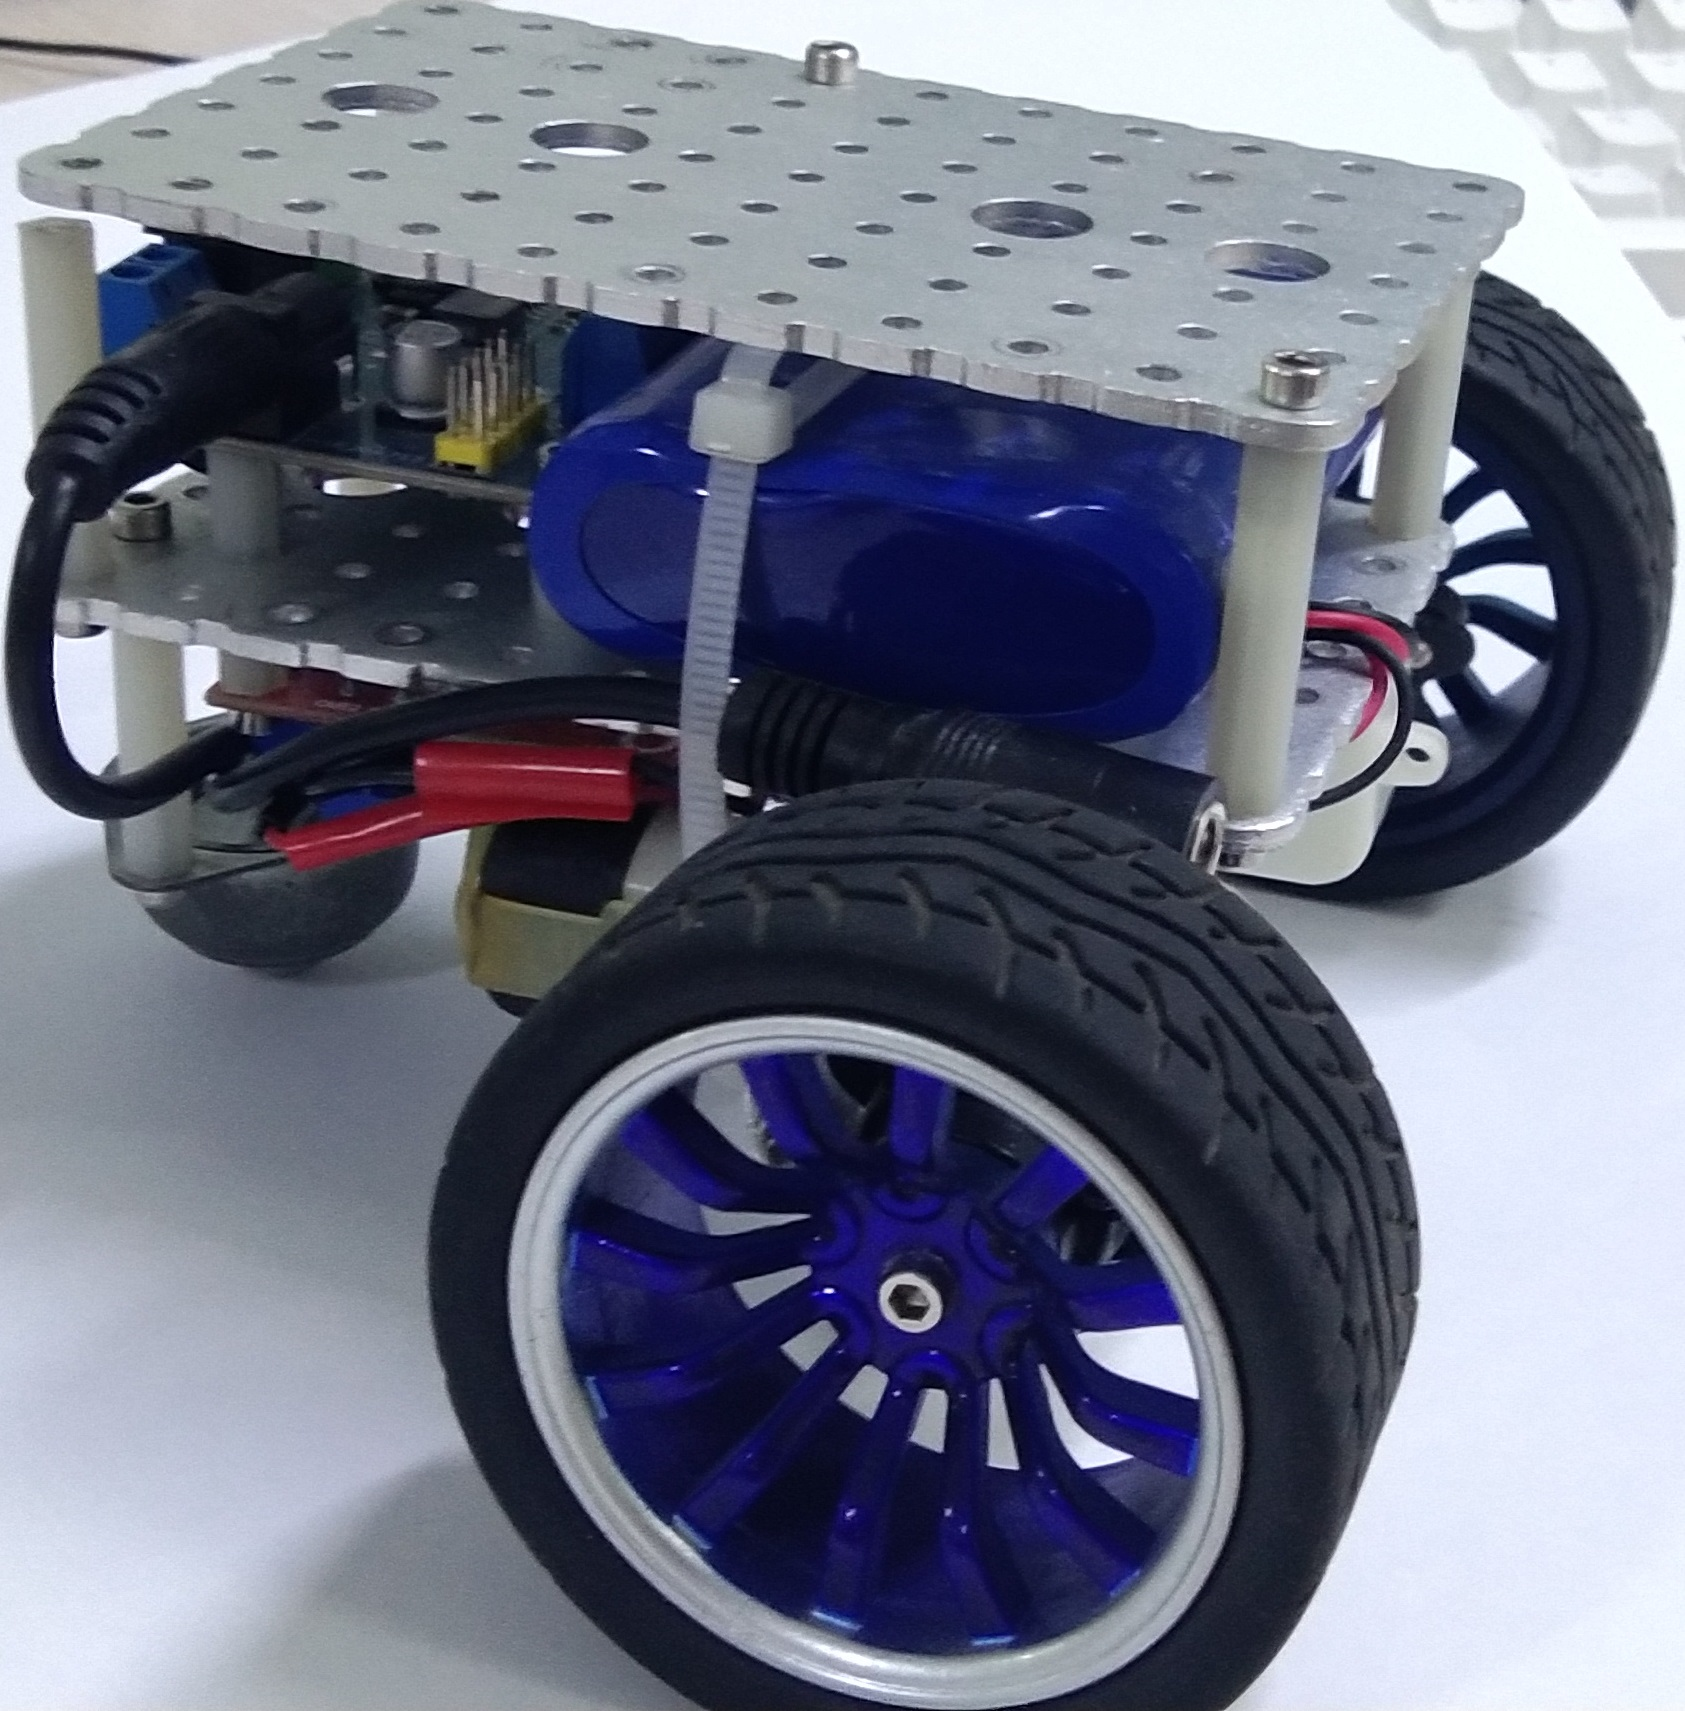
\includegraphics[width=0.5\linewidth]{AGV骨架.jpg}
    \caption{AGV骨架.}
    \label{fig:AGVgj}
\end{figure}

\subsection{xx}
三维结构图如\autoref{fig:zj}(a)所示。图如\autoref{fig:zj}(b)所示。如\autoref{fig:zj}(c)所示。
\begin{figure}[H]
    \centering
    \subfloat[摄像头支架]{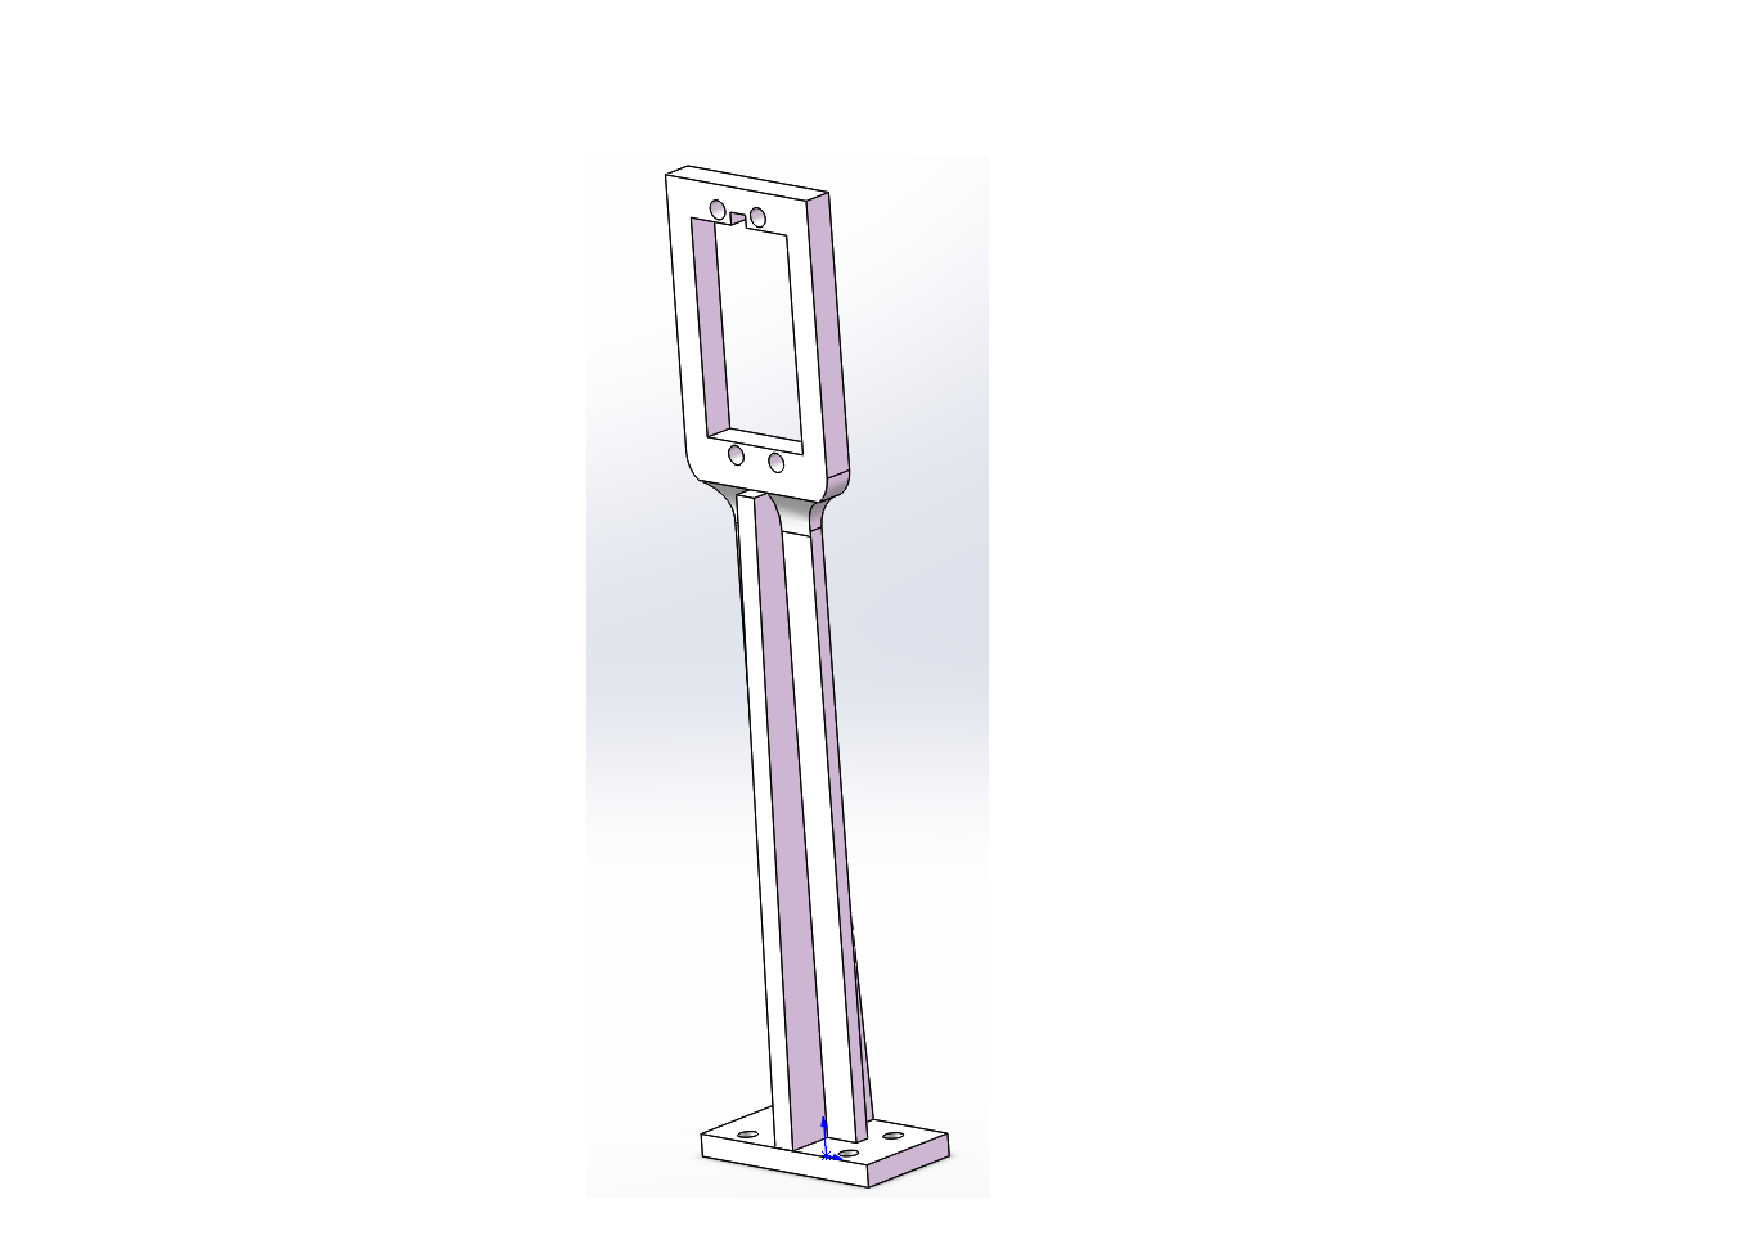
\includegraphics[height=60mm]{摄像头支架.PDF}}
    \hfill
    \subfloat[照相机联轴器]{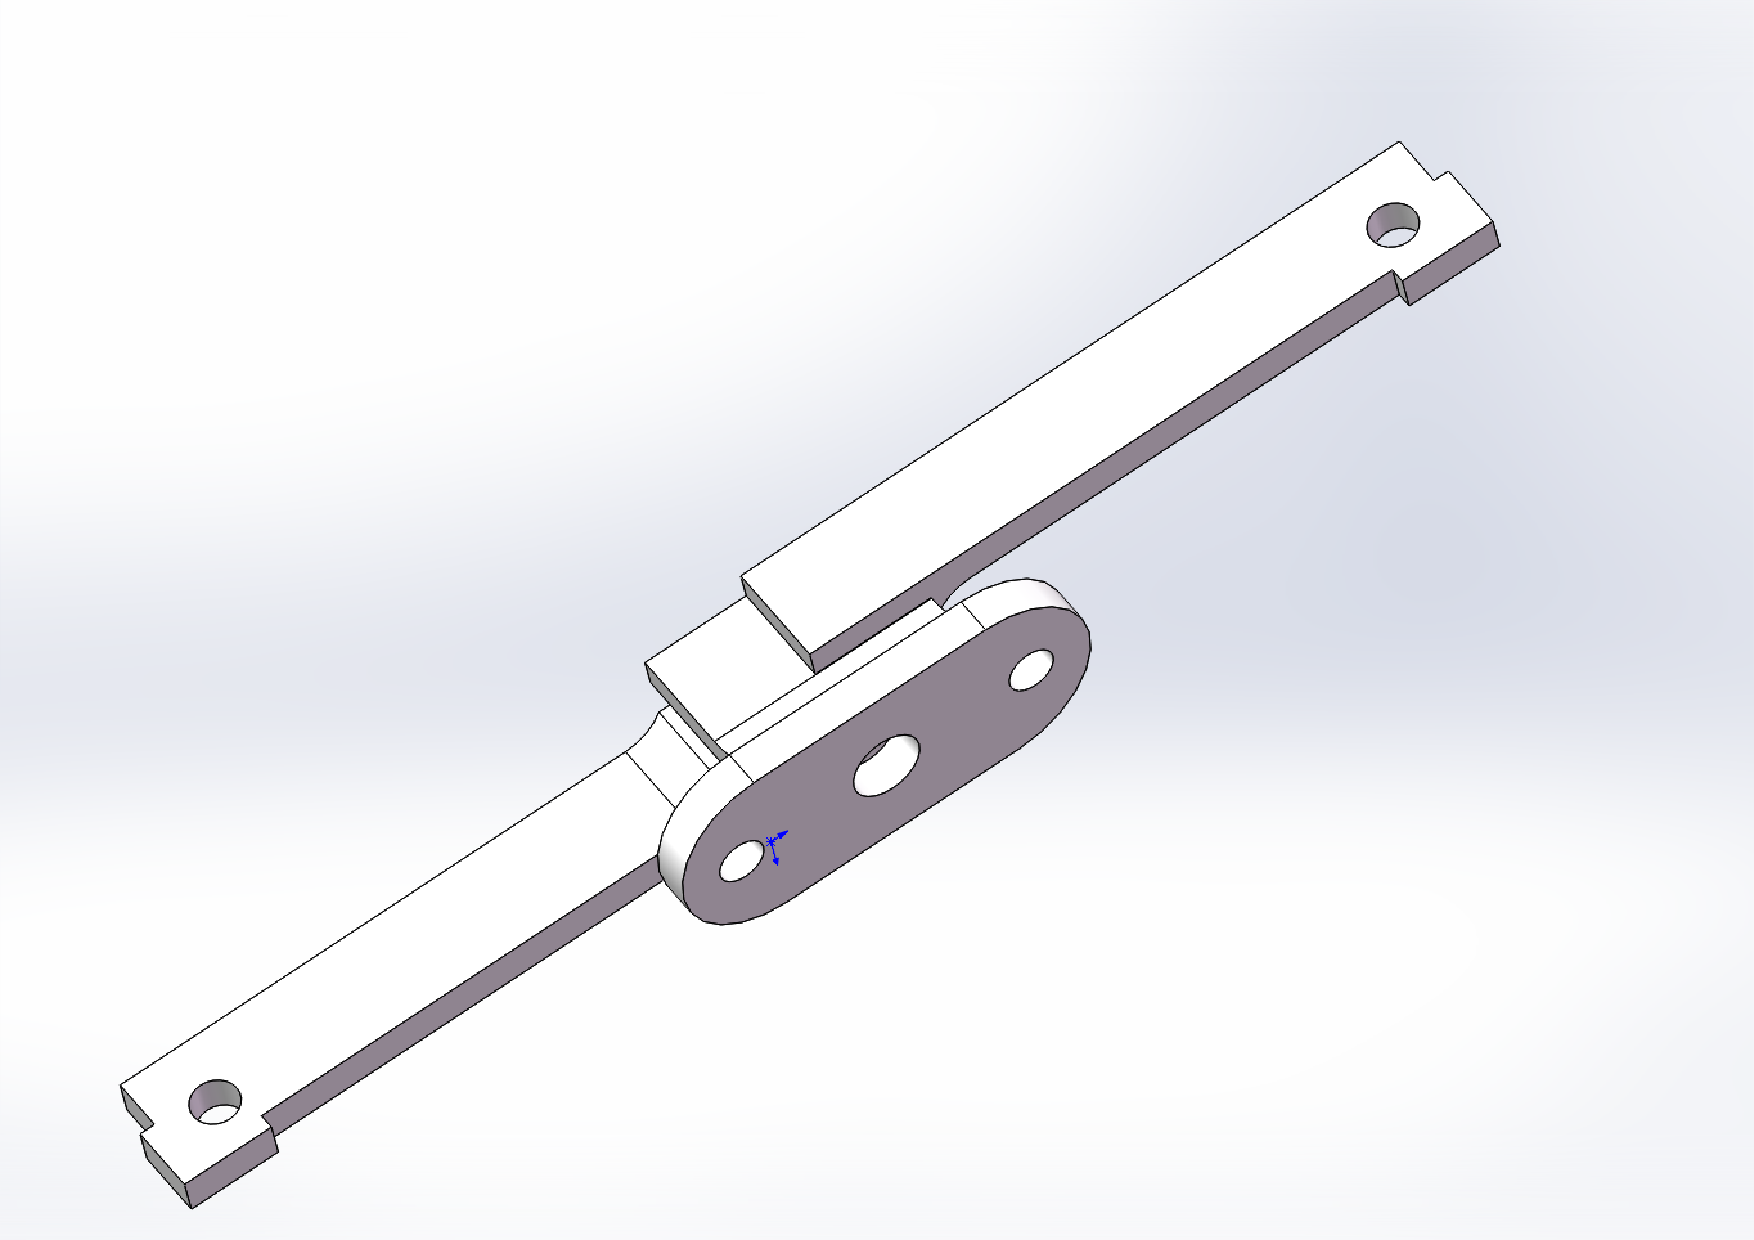
\includegraphics[height=50mm]{照相机联轴器.PDF}}
    \hfill
    \subfloat[支架实体]{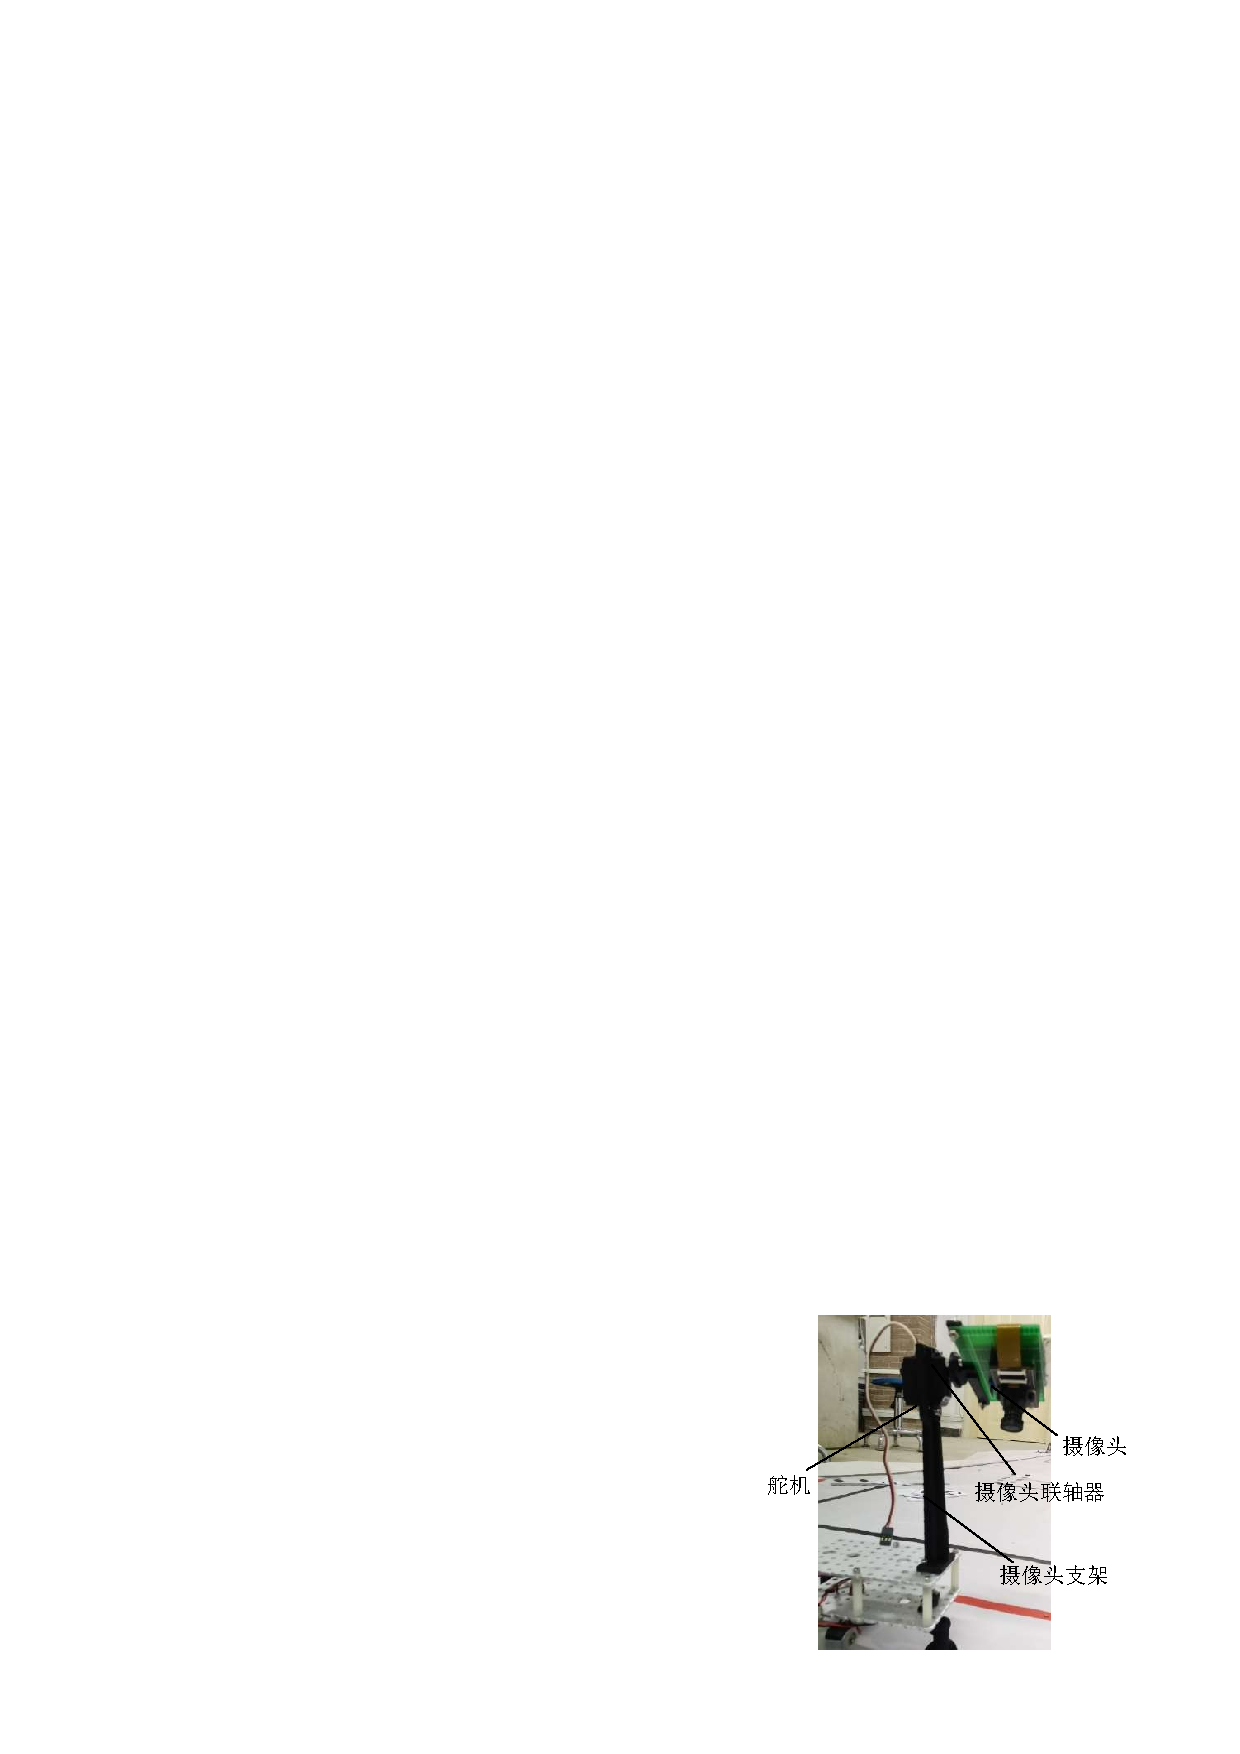
\includegraphics[height=50mm]{支架实体.pdf}}
    \caption{摄像头支架.}
    \label{fig:zj}
  \end{figure}

引脚定义如\autoref{tab:yjdy}
\begin{table}[H]
    \centering
    \small
    \caption{W25Q16引脚定义.}
    \label{tab:yjdy}
    \begin{tabular}{cccc}
    \toprule
    引脚编号 & 引脚名称       & I/O & 功能             \\ \midrule
    1    & /CS        & I   & 片选端输入          \\
    2    & DO(IO1)    & I/O & 数据输出(数据输入输出1)  \\
    3    & /WP(IO2)   & I/O & 写保护输入(数据输入输出2) \\
    4    & GND        & -   & 地              \\
    5    & DI(IO0)    & I/O & 数据输入(数据输入输出0)  \\
    6    & CLK        & I   & 串行时钟输入         \\
    7    & /HOLD(IO3) & I/O & 保持端输入(数据输入输出3) \\
    8    & VCC        & -   & 电源             \\ \bottomrule
\end{tabular}
\end{table}
芯片手册给出的电源域详细说明\footnote{注意:组A、B、C 之间的IO 电源相互不互联,电压可以不一致;相同组内的IO 电源互联,电压一致。}


\section{本章小结}
本章主要...


% 第四章 xxx 

\chapter{xx}
单阶段模型\upcite{liluqiJiYuShenDuXueXiHeBianYuanJianCeDeDongTaiChangJingXiaLuBangSLAM2021},
\section{xx}
xx
\subsection{xx}
xx
\subsection{xx}
\begin{itemize}%[label={$\bullet$}]
    \item xx
    \item xx
    \item xx
    \item xx
    \item xx
\end{itemize}

\section{本章小结}
本章主要介绍了xxx\upcite{xiaosuhua2021,hedongjian2015}

 
% 第五章 xxx  

\chapter{xx}
xx
\section{xx}
\subsection{xx}
xx


% 第六章 xxx 
\chapter{xx}

\section{xx}
\subsection{xx}
xx
输入$e(t)$和输出$u(t)$的关系:
\begin{equation}
    u(t)=K_{p} e(t)+K_{i} \int_{0}^{t} e(\tau) d \tau+K_{d} \frac{d e(t)}{d t}
\end{equation}

所以最终可以得到式\eqref{eqn:51}
\begin{equation}
    \label{eqn:51}
    u(k)=K_{p} e_{k}+K_{i} \sum_{i=1}^{k} e(i) \Delta t+K_{d} \frac{e(k)-e(k-1)}{\Delta t}
\end{equation}


\section{本章小结}
本章节主要介绍了xxx 


% 第七章 xxx 
\chapter{xx}
xxx
\section{xxx}
xxx


\section{本章小结}
本章主要介绍了xxx


% 第八章 xxx 
\chapter{总结与未来展望}
随着科技的快速发展....


% 第九章 xxx  
\chapter{市场与经济分析}

随着科技的快速发展xxx


% 致谢

\backmatter  % 结束章节自动编号

%%%%%%%%%%%%%%%%%%%%%%%%%%% Thanks page %%%%%%%%%%%%%%%%%%%%%%%%%%%%%%%%%%%%

\begin{thankpage}
  % \setlength{\baselineskip}{24pt}

  谢谢你们!谢谢你们!谢谢你们!谢谢你们!谢谢你们!谢谢你们!谢谢你们!谢谢你们!谢谢你们!谢谢你们!谢谢你们!谢谢你们!谢谢你们!谢谢你们!谢谢你们!谢谢你们!谢谢你们!谢谢你们!谢谢你们!谢谢你们!谢谢你们!谢谢你们!谢谢你们!谢谢你们!谢谢你们!谢谢你们!谢谢你们!谢谢你们!谢谢你们!谢谢你们!谢谢你们!谢谢你们!谢谢你们!谢谢你们!谢谢你们!谢谢你们!谢谢你们!谢谢你们!谢谢你们!谢谢你们!谢谢你们!谢谢你们!谢谢你们!谢谢你们!谢谢你们!谢谢你们!谢谢你们!谢谢你们!谢谢你们!谢谢你们!谢谢你们!



\end{thankpage}


% 参考文献
%%%%%%%%%%%%%%%%%%%%%%%% 生成参考文献 %%%%%%%%%%%%%%%%%%%%%%%%%%%%%%%%%%%%%

% 生成参考文献, 使用第一种请把第二种全部注释

% 第一种方式, 使用 bib 文件

%\nocite{*}  % 可以暂时显示全部参考文献, 包括未引用的

% 使用方法:\bibliography{参考文件1文件名, 参考文献2文件名, ...}
% 参考文献格式可选  plain, abbrv, unsrt, siam

% \bibliographystyle{thuthesis-numeric}
\titleformat{\chapter}{\centering \fontsize{15pt}{23pt}\selectfont \bfseries\heiti}{}{0em}{}
\bibliography{mybib}
% 第二种方式, 按照格式直接写文献信息, 使用第二种请把第一种全部注释
% 注意: 第二种方式需要加下面三行命令才能把  "参考文献 " 加到目录
% \clearpage
% \phantomsection
% \addcontentsline{toc}{chapter}{参考文献} % 添加  "参考文献 " 到目录

% \begin{thebibliography}{99}

% \bibitem{Adams2003} Adams~R~A, Fournier~J~J~F. Sobolev spaces. Elsevier, 2003.

% \bibitem{Shen1994} Shen~J. Efficient spectral-Galerkin method I. Direct solvers of second- and fourth-order equations using Legendre polynomials. SIAM J. Sci. Comput., 1994, 15(6): 1489-1505.

% \bibitem{Tadmor2012} Tadmor~E. A review of numerical methods for nonlinear partial differential
%  equations. Bull. Amer. Math. Soc., 2012, 49(4): 507-554.

% \bibitem{TreWei2014}Trefethen~L~N, Weideman~J~A~C. The exponentially convergent trapezoidal rule. SIAM Rev., 2014, 56(3): 385-458.

% \bibitem{LiLiu1997} 李荣华, 刘播. 微分方程数值解法. 东南大学出版社, 1997.

% \end{thebibliography}


% 本科成就
\begin{achievement}
    {%
        \noindent \heiti \zihao{-4} \textbf{科研项目} 
        
        \noindent [1] xxx

        \noindent [2] xxx
        
        \noindent \heiti \zihao{-4} \textbf{发表论文}
        
        \noindent [1] xxx

        \noindent [2] xxx

        \noindent [3] xxx

        \noindent \heiti \zihao{-4} \textbf{专利}

        \noindent [1] xxx

        \noindent \heiti \zihao{-4} \textbf{科技竞赛}

        \noindent \heiti \zihao{-4} \textbf{国家级:}

        \noindent [1] xxx

        \noindent [2] xxx

        \noindent [3] xxx

        \noindent [4] xxx

        \noindent [5] xxx
        
        \noindent \heiti \zihao{-4} \textbf{省级:}

        \noindent [1] xxx

        \noindent [2] xxx

        \noindent [3] xxx

        \noindent [4] xxx

        \noindent [5] xxx

    }
    \end{achievement}


% 附录
%%%%%%%%%%%%%%%%%%%%%%%% 附录 %%%%%%%%%%%%%%%%%%%%%%%%%%%%%%%%%%%%%%%

% 添加附录, 如不需要可以注释掉
\appendix

% 附录正文
% \chapter{\centerline{附录 A ~ 这是第一个附录}}
\clearpage
\phantomsection
\addcontentsline{toc}{chapter}{附录 A ~ 总原理图}
\vspace*{-1.5ex}
\begin{center} \heiti \chpzihao \bfseries 附录 A ~ 总原理图 \end{center}
\chaptermark{附录 A ~ 总原理图}


\renewcommand{\thesection}{A.\arabic{section}}


\clearpage
\phantomsection
\addcontentsline{toc}{chapter}{附录 B ~ 关键程序}
\vspace*{-1.5ex}
\begin{center} \heiti \chpzihao \bfseries 附录 B ~ 关键程序 \end{center}
\chaptermark{附录 B ~ 关键程序}
\renewcommand{\thesection}{B.\arabic{section}}
\section{python}
\begin{python}
import sensor
import image
import lcd
import KPU as kpu
import time
from fpioa_manager import fm
from machine import UART
import gc


\end{python}
\section{C}
\begin{c++}
#include "TrackCar.h"
#include "bsp_tb6612.h"
#include "bsp_gpio.h"
#include "motor_ctrl.h"
#include "bsp_spi_nrf.h"
#include "RecvBuffer.h"
#include "SendPack.h"

\end{c++}


\end{document}








% \section{算法环境}

% 如下是算法~\ref{alg:euclid}.
% \begin{algorithm}[H]
%     \small
%     \caption{Euclid's algorithm}\label{alg:euclid}
%     \begin{algorithmic}[1]
%         \Procedure{Euclid}{$a,b$}\Comment{The g.c.d. of a and b}
%         \State $r\gets a\bmod b$
%         \While{$r\not=0$}\Comment{We have the answer if r is 0}
%         \State $a\gets b$
%         \State $b\gets r$
%         \State $r\gets a\bmod b$
%         \EndWhile\label{euclidendwhile}
%         \State \Return $b$\Comment{The gcd is b}
%         \EndProcedure
%     \end{algorithmic}
% \end{algorithm}


% \clearpage
% 如下是算法~\ref{alg:name}, 算法宽度可以通过 minipage 宏包调节.
% \begin{center}
% \vspace{-2ex}
% \begin{minipage}{.9\linewidth}
% \begin{algorithm}[H]
% \caption{算法的名字}\label{alg:name}  % 算法的名字
% \begin{algorithmic}[1]
% \Require  input parameters A, B, C  % 算法的输入
% \Ensure  output result   % 算法的结果输出
% \State some description 算法介绍   % \State 后写一般语句
% \For{condition}    % For 语句,需要和 EndFor对应
%   \State ...
%   \If{condition}  % If 语句,需要和 EndIf对应
%     \State ...
%   \Else
%     \State ...
%   \EndIf
% \EndFor
% \While{condition}  % While语句,需要和 EndWhile对应
%   \State ...
% \EndWhile
% \State \Return result
% \end{algorithmic}
% \end{algorithm}
% \end{minipage}
% \end{center}
